\section{System architecure}
\label{sec:system_architecture}

In this section, we present the architecture of \SeeDB\ starting with an
overview, followed by a detailed discussion of the various modules in \SeeDB.

\subsection{\SeeDB\ architecture overiew}
\label{subsec:overview}

Our prototype of \SeeDB\ is designed as a layer on top of a relational database
system.
While optimization opportunities are restricted by virtue of being outside the
database, our design permits \SeeDB\ to be used in conjunction with a variety of
existing database systems. \SeeDB\ is comprised of two main parts: the \SeeDB\
front end and the \SeeDB\ backend. The front end is a ``thin client'' that
is only used to issue queries to \SeeDB\ and view results. The backend in
contrast performs all the computation required to generate and select views. Figure \ref{fig:sys-arch}
shows the architecture of our system.

\begin{figure}[htb]
\centerline{
\hbox{\resizebox{9cm}{!}{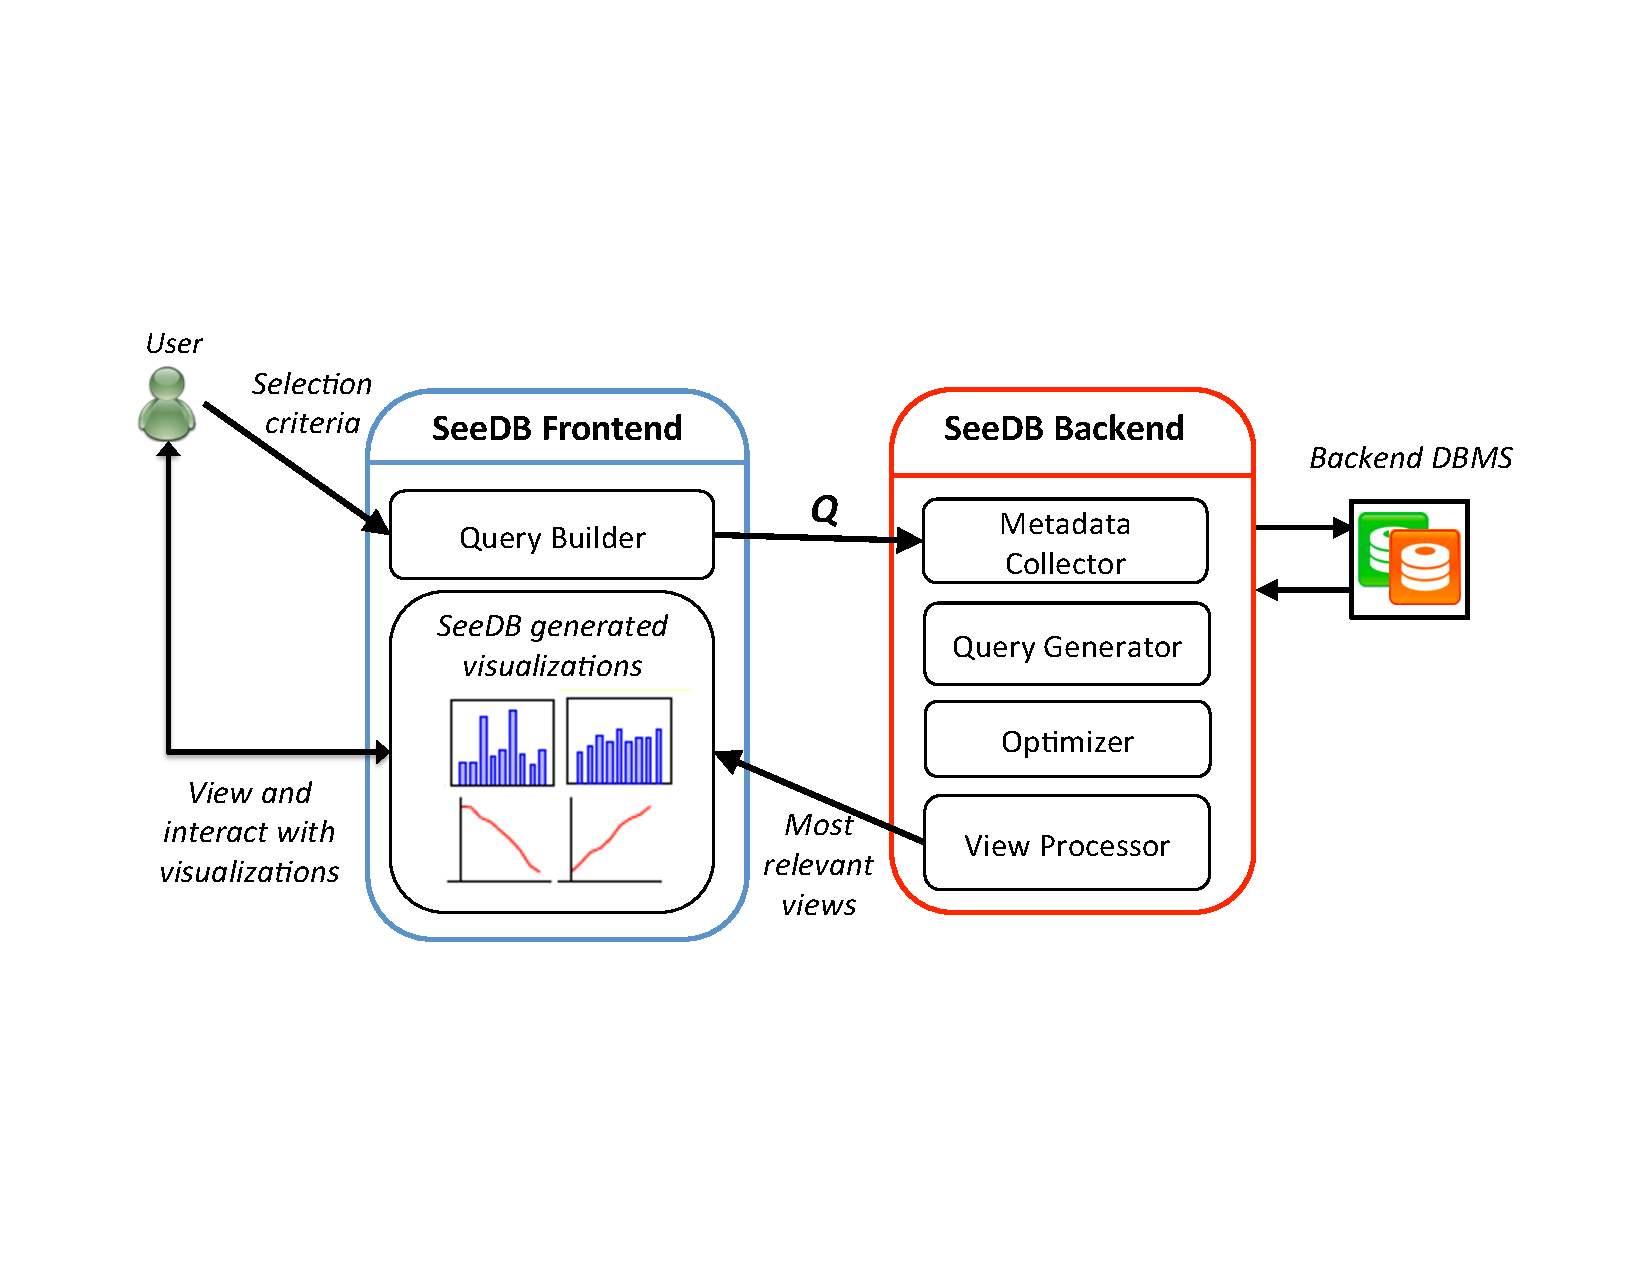
\includegraphics[trim=10mm 50mm 10mm 50mm,
clip=true]{Images/seedb-architecture.pdf}}}}
\caption{SeeDB Architecture}
\label{fig:sys-arch}
\end{figure} 

An analyst uses the front end to issue queries to \SeeDB. We provide three
mechanisms for the analyst to issue queries: raw SQL, an intuitive
query-builder, and a set of pre-formulated queries for common operations on a
dataset (we discuss query input further in Section \ref{subsec:seedb_frontend}).
Once the analyst issues a query via the \SeeDB\ front end, the backend
takes over.
First, the Metadata Collector module queries metadata tables (a combination of
database-provided and \SeeDB\ specific tables) for information such as table
sizes, column types, data distribution, and table access patterns.
The resulting metadata along with the analyst's query is then passed to the
Query Generator module. The purpose of the Query Generator is two-fold:
first, it uses the metadata obtained in the previous step to prune the space of
candidate views to the most promising ones; and second, it generates target and
comparison views for each view that has not been pruned.
The SQL queries corresponding to the target and comparison views are then passed
to the Optimizer module. We refer to these queries collectively as {\it view
queries}.
The Optimizer module is responsible for determining the best way to combine
view queries intelligently so that the total execution time is
minimized. 
(We discuss the optimizations performed by the Query Generator and
Optimizer modules further in Section \ref{subsec:seedb_backend}.) Once the
Optimizer module has generated the optimized queries, \SeeDB\ sends the
queries to the underlying database system for execution. The results returned by
the DBMS are then processed by the View Processor module. This module processes
results of the optimized queries in a streaming fashion and produces results for
individual views. Results of individual views are then normalized as discussed
in Section~\ref{sec:problem_statement} and the utility of each view is computed.
Finally \SeeDB\ selects the top $k$ views with the highest utility and returns them to the
\SeeDB\ front end which creates visualizations for each view and displays
the visualizations to the analyst.

We now discuss the \SeeDB\ modules in detail.

\subsection{SeeDB Frontend}
\label{subsec:seedb_frontend}

The \SeeDB\ frontend serves a two-fold purpose: allow the analyst to input a
query, and to visualize the results (views) produced by the \SeeDB\ backend.
As mentioned before, we provide the analyst with three options for specifying an
input query: (a) as raw SQL, (b) through a query builder that can allow users
unfamiliar with SQL to formulate queries through an easy-to-use form-based
interface, (c) through pre-defined query templates to perform common operations
on a dataset, e.g., select outliers in a particular column. These
templates are particularly useful since users are often interested in anomalous
data points.

Once the analyst issues a query via the \SeeDB\ frontend, the \SeeDB\ backend
evaluates various views and sends the most interesting ones back to the
frontend.
For each view in the result, the \SeeDB\ frontend determines the best
way to visualize the view depending on parameters including the data
type being represented and the number of distinct values. 
The resulting
visualizations are displayed to the analyst who can then examine
these ``most interesting'' views at a glance, explore specific views in detail and
view metadata for each view (e.g. size of result, sample data, value with
maximum change and other statistics). 
The user can also slice-and-dice views further by performing drill-downs on the 
relevant attributes in the view. 
%This action automatically
%modifies the selection query and displays views for the subset of data
% selected. The user can of course revert back to the original views and continue exploring the data.

\subsection{SeeDB Backend}
\label{subsec:seedb_backend}

As discussed in Section \ref{subsec:overview}, \SeeDB\ is implemented using a
light-weight frontend described in the previous section and a backend that
performs all the computations for generating and selecting views. Furthermore,
as shown in Figure~\ref{fig:sys-arch}, the \SeeDB\ backend is composed of four
modules that are respectively responsible for collecting metadata (Metadata Collector), pruning
the view space and generating view queries (Query Generator), optimizing view
queries (Optimizer), and processing query results to identify the top-$k$
interesting views (View Processor). In this section, we will discuss the various
techniques underlying \SeeDB. To achieve its goal of finding the most
interesting views accurately and efficiently, \SeeDB\ must not only accurately
estimate the accuracy of a large number of views but also design ways in which
the total processing time will be minimized.
We first describe the basic \SeeDB\ framework and then briefly discuss our optimizations.

% One of the chief challenges in \SeeDB\ is producing the most interesting views
% of the query result in the least possible time. For achieve the above
% performance goal, \SeeDB\ must perform optimizations at two stages: first, using
% prior knowledge such as statistics to prune out uninteresting views without examining table data; and second, minimizing the
% execution time for queries that are issued to the database. 

\subsubsection{Basic Framework}
\label{subsubsec:basic_framework}

Given a user query $Q$, the basic technique used in \SeeDB\ computes all
possible views obtained by adding a single aggregate and a single group-by
clause to $Q$. Target and comparison views corresponding to each view are
computed and each view query is executed independently on the DBMS. The
results for each view are then computed and the utility of the view is
computed by comparing the target view distribution and the comparison view
distribution (Section \ref{sec:problem_statement}). Finally, the top-$k$ views
with the largest utility are chosen. The basic approach is clearly inefficient
since it examines each possible view and executes each view query independently;
we next discuss how our optimizations fix some of these problems.

\subsubsection{View Space Pruning}
\label{subsubsec:view_space_pruning}

Most views possible for any query $Q$ have low utility since the target view
distribution is very similar to the comparison view distribution. 
As a result,
\SeeDB\ aggressively prunes view queries that are unlikely to have high
utility. 
This pruning is based on metadata about the table including data
distributions and access patterns for the table. (This information is collected
by the Metadata Collector module.)
 Specifically, we use variance estimates for
table columns and correlation measures between columns of the table. 
If two columns in the table have high correlation, the views generated by grouping with respect to these two
columns will be very similar. 
We therefore only generate a single view for the
pair of columns. 
We can similarly use statistical properties of measure
attributes to prune views further. 
Finally, if access patterns for the table are
available, we can use them to prune views with attributes that are
rarely accessed and are therefore likely to be unimportant.

\subsubsection{View Query Optimizations}
\label{subsubsec:optimizations}

The second set of optimizations used by \SeeDB\ minimizes the execution time for
view queries that haven't been pruned using the techniques described above.
Since view queries are very similar (e.g. target and comparison views only differ in the subset of data that the
query is run on) \SeeDB\ uses multiple techniques to combine view queries. 
The ultimate goal is to minimize scans of the underlying dataset by sharing as
many table scans as possible. Our optimization strategies include:

\begin{enumerate}
  \item {\it Combine target and comparison view}: Since the target view and
  comparison views only differ in the subset of data that the query is
  executed on, we combine the two queries to generate these view into one.
  This simple optimization halves the time required to compute the results for
  a single query.
  \item {\it Combine Multiple Aggregates}: A large number of view
  queries have the same group-by clause but aggregates over different attributes.
  Therefore, \SeeDB\ combines all view queries with the same group-by clause
  into a single view query. This rewriting provides a speed up linear in the
  number of aggregate attributes.
  \item {\it Combine Multiple Group-bys}: 
  \SeeDB\ computes a large number of group-bys. One optimization is to
  combine queries with different group-by attributes into a single query with
  multiple group-bys attributes. For instance, consider view queries $V(Q,
  A_1,$ $G_1)$, $V(Q, A_1,$ $G_2)$ \ldots $V(Q, A_1,$ $G_n)$. Instead of
  executing them individually, we can rewrite them into a single view query
  $V(Q, A_1,$ $(G_1, G_2$\ldots $G_n))$. While this optimization can reduce the
  number of queries executed, the number of group by attributes we can include in a single query
  depends on the correlation between values of the various attributes (this
  affects number of distinct groups) and the working memory. We compute the
  optimal combinations of group-bys by modeling the problem as a variant of
  bin-packing (We discuss our algorithm in our full paper~\ref{}). 
%   A variation of this approach also implemented
%   on \SeeDB\ is to send the results of the multiple group-by query to the front
%   end and ask the \SeeDB\ frontend to compute utility and select views. The
%   advantage of this approach is that it allows for more efficient interactive
%   exploration of the views.
  \item {\it Sampling}: The optimization that can have the most impact in
  terms of efficiency is to reduce the number of tuples examined by
  constructing a data sample and running all queries against the sample. As
  expected, the sampling technique and size of the sample significantly affects
  the accuracy of the generated views. 
\end{enumerate}

%\begin{figure}[htb]
%\centerline{
%\hbox{\resizebox{9cm}{!}{\includegraphics[trim=10mm 50mm 10mm 50mm,
%clip=true]{Images/seedb-frontend.pdf}}}}
%\caption{SeeDB Frontend}
%\label{fig:frontend}
%\end{figure} 


